\documentclass[12pt,letterpaper]{article}
\usepackage[margin=1in]{geometry}
\usepackage{tabularx}
\usepackage{float}
\usepackage{graphicx}
\usepackage{amsmath}
\usepackage{amsfonts}
\title{Project 1}
\author{Owen Sowatzke}
\date{October 10, 2022}

\begin{document}
\maketitle
\section{LFM Parameters:}
A pulsed radar system was generated in MATLAB using the following parameters:
\begin{table}[H]
\caption{Radar System Parameters}
\label{Parameter Table}
\begin{tabularx}{\textwidth}{| X | X |}
\hline
Carrier Frequency & 10 GHz \\
\hline
Sample Rate & 100 MHz \\
\hline
Transmit Power & 20 dB \\
\hline
Antenna Gain & 44.15 dB \\
\hline
Noise Figure & 10 dB \\
\hline 
System Losses & 5 dB \\
\hline
PRF & 50 kHz \\
\hline
Duty Cycle & 20\% \\
\hline
Chirp Bandwidth & 100 MHz \\
\hline
\end{tabularx}
\end{table}
\noindent
Using the parameters given in Table \ref{Parameter Table}, the radar system's PRI can be computed as follows:
\begin{equation}
PRI = \frac{1}{PRF} = 20 {\mu}s
\label{PRI Equation}
\end{equation}
Let the radar system's duty cycle be given by $D$. Then, the length of the LFM pulse ($\tau$) is given as follows:
\begin{equation}
\tau = PRI \cdot D = 4 {\mu}s
\label{tau equation}
\end{equation}
\section{System Modeling}
To simulate the given radar system, the received signal for each of the target returns must be generated. This received signal is then passed through a matched filter to increase the SNR of the target returns.
\subsection{Modeling the Received Signal}
The received signal is generated according to the block diagram given in Fig. \ref{Generate RX Sig}.
\begin{figure}[H]
\center{\fbox{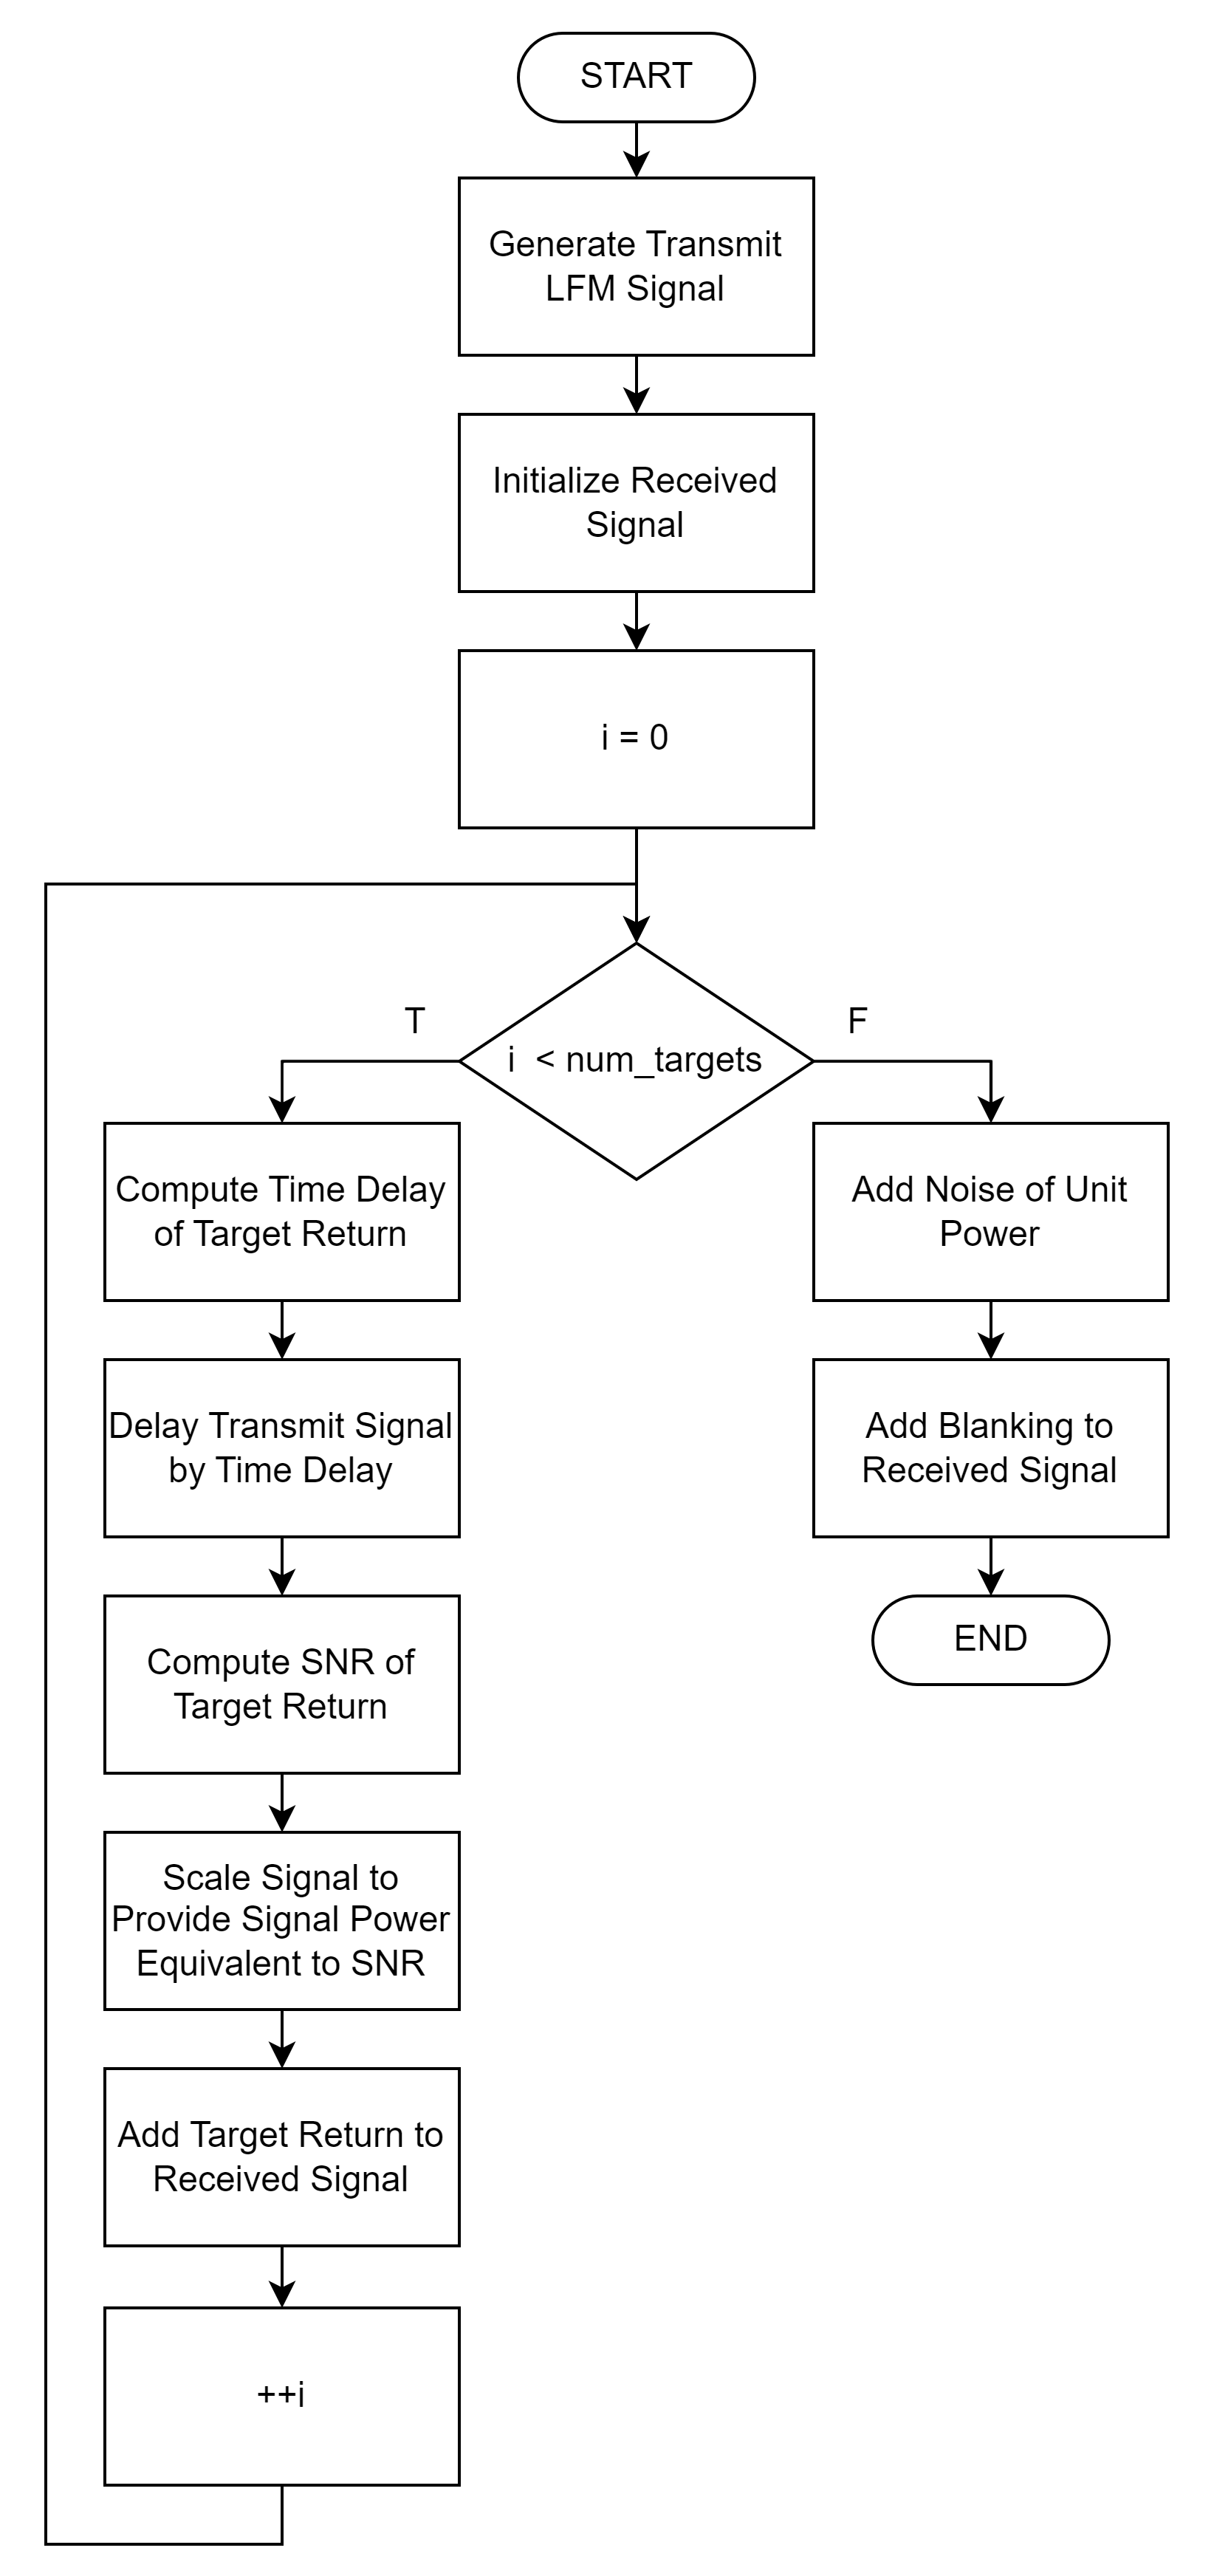
\includegraphics[width=0.5\textwidth]{gen_rx_sig.png}}}
\caption{Generating Received Signal}
\label{Generate RX Sig}
\end{figure}
\noindent
The transmitted signal is an LFM waveform padded with zeros to length of the pulse. The LFM waveform is generated using the following formula:
\begin{equation}
x(t) = e^{j\pi \beta t^2/\tau}
\label{lfm_equation}
\end{equation}
where $\beta$ is the bandwidth of the chirp waveform and $\tau$ is the length of the chirp waveform. The received signal is generated using a scaled and delayed versions of the transmitted signal. The delay of each target can be computed using the following formula:
\begin{equation}
t_d = \frac{2R}{c}
\end{equation}
Each of the target returns is then scaled to provide an SNR given by the following formula:
\begin{equation}
SNR = \frac{P_t G^2 \lambda^2 \sigma}{(4\pi)^3 R^4 k T_0 B_n F_n L_s L_\alpha(R)}
\end{equation}
The noise has unit power. Therefore, to provide the required SNR, each of the target returns must be scaled by $10^{SNR/20}$. The received signal is the sum of each of the target returns and noise. Assuming the radar system has a duplexer, the received signal will also have blanking (i.e. during transmission the receiver will not receive any signal). To model this blanking, the first $L$ samples of the received signal are replaced with zeros.
\subsection{Modeling the Matched Filter}
The matched filter output is generated according to the block diagram shown in Fig. \ref{Generate MF Output}.
\begin{figure}[H]
\center{\fbox{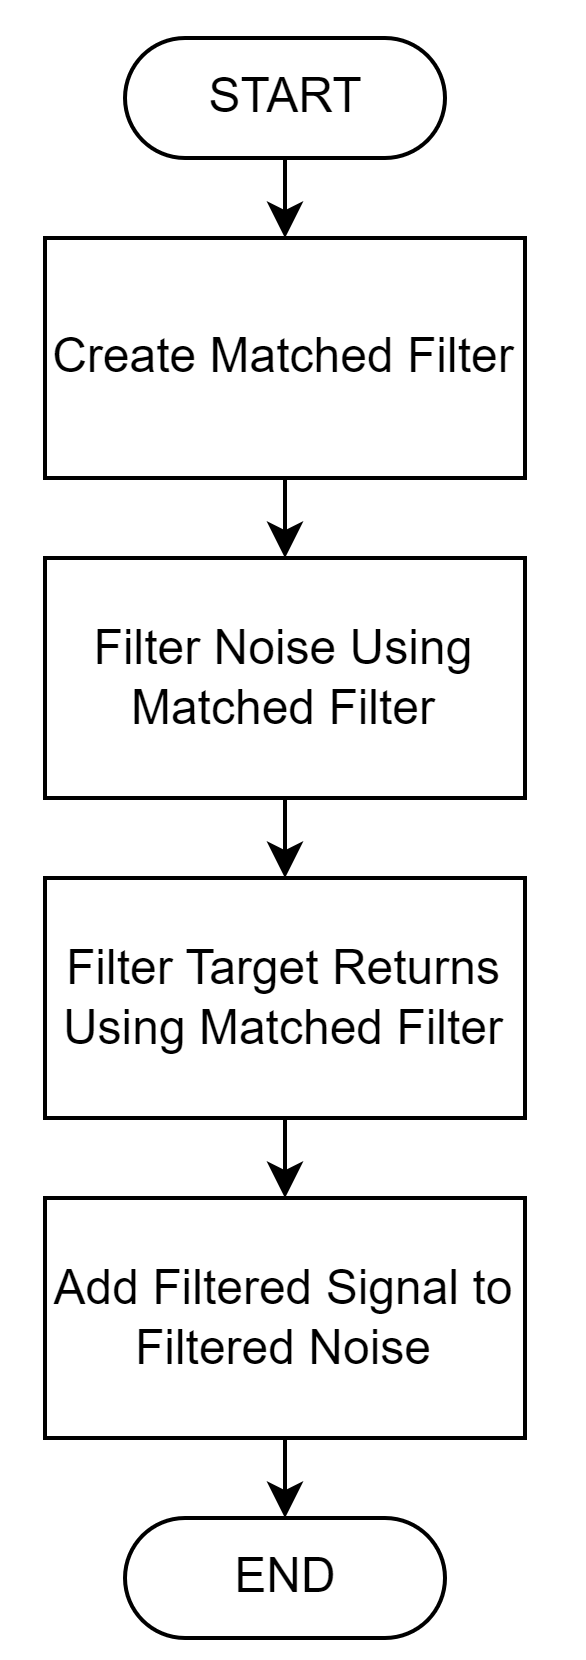
\includegraphics[width=0.2\textwidth]{gen_mf_output.png}}}
\caption{Generating Matched Filter Output}
\label{Generate MF Output}
\end{figure}
\noindent
The matched filter is generated according to the following formula:
\begin{equation}
h(t) = x^*(T_M - t)
\end{equation}
where $x(t)$ is given in equation \eqref{lfm_equation} and $T_M$ is the duration of the LFM pulse. Convolution is a linear operator. As such, the matched filter operation can be expressed in the following manner:
\begin{equation}
y(t) = h(t) * (x(t) + n(t)) = h(t)*x(t) + h(t)*n(t)
\end{equation}
The noise and signal can be filtered idependently and produce the same matched filter result. This approach is leveraged in the simulation, and it enables the SNR of the matched filter to be more easily extracted.
\section{Matched Filter SNR}
The SNR of a target return can be examined at the ADC and after the matched filter. The SNR of the matched filter output should by larger than the SNR of the ADC input by a factor of the filter length. This result will be confirmed via MATLAB simulation.
\subsection{SNR of the Received Signal}
A single target is placed at a time delay  of $25\%$ of the PRI or $5\mu s$. This time delay corresponds to a target at a range of
\begin{equation}
R = \frac{ct_d}{2} = 750 m
\end{equation}
The radar cross section of this target is scaled to provide an SNR of $20dB$. The radar cross section corresponding to this SNR is
\begin{equation}
\sigma = \frac{(4\pi)^3 R^4 k T_0 B_n F_n L_s L_\alpha(R)\cdot SNR}{P_t G^2 \lambda^2} = 0.01307 m^2
\end{equation}
The received signal can be generated by inserting these parameters into the block diagram shown in Figure \ref{Generate RX Sig}. The received signal that results is shown in Figure \ref{ADC Sig}.
\begin{figure}[H]
\center{\fbox{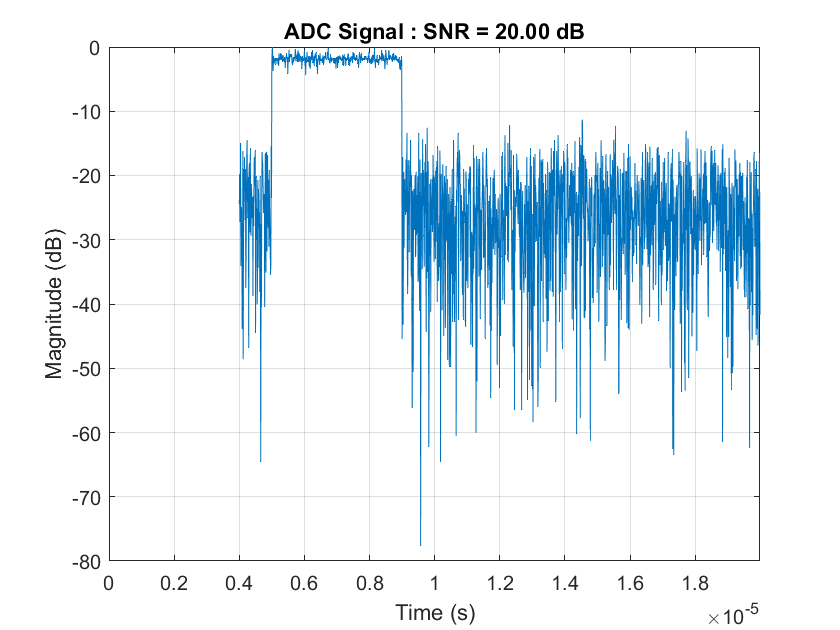
\includegraphics[width=0.5\textwidth]{adc_sig.png}}}
\caption{Received Signal}
\label{ADC Sig}
\end{figure}
\subsection{SNR of the Matched Filter Output}
The matched filter output is generated according to the block diagram shown in Figure \ref{Generate MF Output}. Let $x[n]$ be the matched filter. Then, the power of the matched filter output ($x[n]$) is given by the following equation:
\begin{equation}
P_s = max(|x[n]|)^2
\end{equation}
Now, let $x[n]$ define the noise after the matched filter (ignoring the blanking and filter chargeup). Then, the power of the noise after the matched filter is given by the following equation:
\begin{equation}
P_n = \frac{1}{N}\sum_{n=0}^{N-1}|x[n]|^2
\end{equation}
Finally, the SNR at the output of the matched filter is given by
\begin{equation}
SNR = 10log_{10}\frac{P_s}{P_n}
\end{equation}
The theoretical SNR of the matched filter output should be greater than the SNR of the received signal by a factor of the filter length. As such the theoretical SNR of the matched filter output is given by
\begin{equation}
SNR = 20 + 10log_{10}L = 46.02 dB
\end{equation}
The output of the matched filter and corresponding SNR are shown in Figure \ref{MF Output}.
\begin{figure}[H]
\center{\fbox{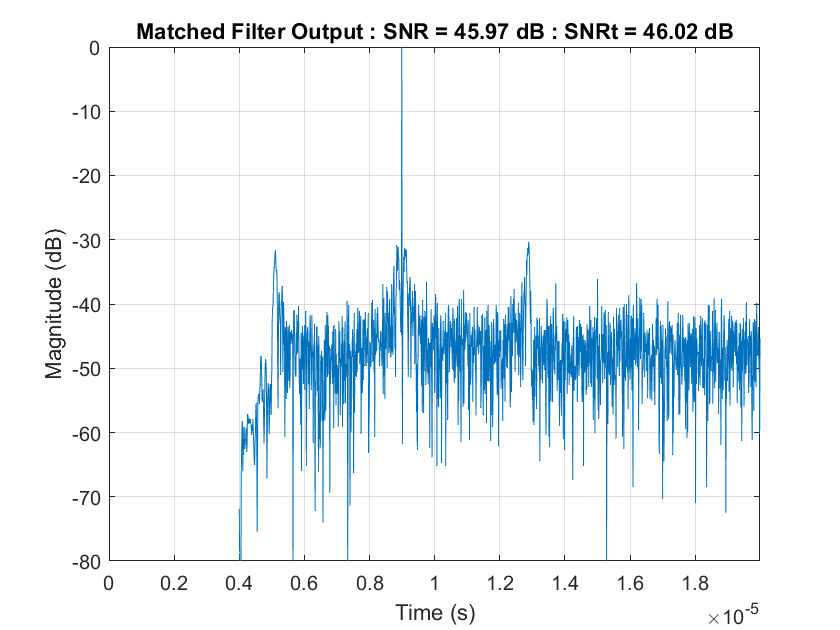
\includegraphics[width=0.5\textwidth]{mf_output.png}}}
\caption{Matched Filter Output}
\label{MF Output}
\end{figure}
\noindent
The SNR of the matched filter output shown in Figure \ref{MF Output} is close to the theoretical SNR. The peak sidelobe level of the matched filter output is approximately $30 dB$. Note that this is lower than the expected $13.26 dB$ sidelobe of a sinc function. This is because the selected LFM waveform is a zadoff chu sequence. 
\begin{equation}
x_u[n] = e^{-j\pi un(n + c_f + 2q)/N_{ZC}}
\end{equation}
where 
$$ 0 \leq n < N_{ZC} $$
$$ 0 < u < N_{ZC} \text{ and } gcd(N_{ZC},u) = 1$$
$$ c_f = N_{ZC} \text{ mod } 2$$
$$ q \in {\mathbb{Z}}$$
\end{document}
